\begin{center}
	\Huge
	Landmåling
\end{center}

Vi skal ud og måle vinkler i gården og på fodboldbanen. Efterfølgende skal I bruge sinus- og cosinusrelationerne til at bestemme længderne på følgende figur.

\begin{figure}[H]
	\centering
	\begin{tikzpicture}
		\node[color = olive, anchor = east] at (0.8,-3) {Flagstang};
		\node[color = olive, anchor = east] at (0.8,-6) {Net};
		\filldraw[color = teal] (0,0) circle (2pt);
		\filldraw[color = teal] (3,0) circle (2pt);
		\filldraw[color = teal] (12,-16.5) circle (2pt);
		\filldraw[color = teal] (3,-5) circle (2pt);
		\filldraw[color = teal] (4,-9) circle (2pt);
		\filldraw[color = teal] (5,-10) circle (2pt);
		\filldraw[color = teal] (0,-9.5) circle (2pt);
		\filldraw[color = teal] (0,-14) circle (2pt);
		\filldraw[color = teal] (1,-16.5) circle (2pt);
		\filldraw[color = teal] (13,-10) circle (2pt);
		\draw[color = teal, thick] (0,0) -- (3,0) node[midway, anchor = south] {$19.7$m};
		\draw[color = teal, thick] (0,0) -- (0.8,-3);
		\draw[color = teal, thick] (0.8,-3) -- (3,0);
		\draw[color = teal, thick] (0.8,-3) -- (3,-5);
		\draw[color = teal, thick] (3,0) -- (3,-5);
		\draw[color = teal, thick] (0.8,-3) -- (0.8,-6);
		\draw[color = teal, thick] (0.8,-6) -- (3,-5);
		\draw[color = teal, thick] (0.8,-6) -- (4,-9);
		\draw[color = teal, thick] (3,-5) -- (4,-9);
		\draw[color = teal, thick] (0.8,-6) -- (0,-9.5);
		\draw[color = teal, thick] (0,-9.5) -- (4,-9);
		\draw[color = teal, thick] (0,-9.5) -- (0,-14);
		\draw[color = teal, thick] (0,-14) -- (1,-16.5);
		\draw[color = teal, thick] (0,-14) -- (4,-9);
		\draw[color = teal, thick] (4,-9) -- (5,-10);
		\draw[color = teal, thick] (0,-14) -- (5,-10);
		\draw[color = teal, thick] (1,-16.5) -- (5,-10);
		\draw[color = teal, thick] (1,-16.5) -- (12,-16.5);
		\draw[color = teal, thick] (5,-10) -- (12,-16.5);
		\draw[color = teal, thick] (12,-16.5) -- (13,-10);
		\draw[color = teal, thick] (5,-10) -- (13,-10);
		\filldraw[color = olive] (0.8,-3) circle (2pt);
		\filldraw[color = olive] (0.8,-6) circle (2pt);
	\end{tikzpicture}
\end{figure}

\begin{center}
	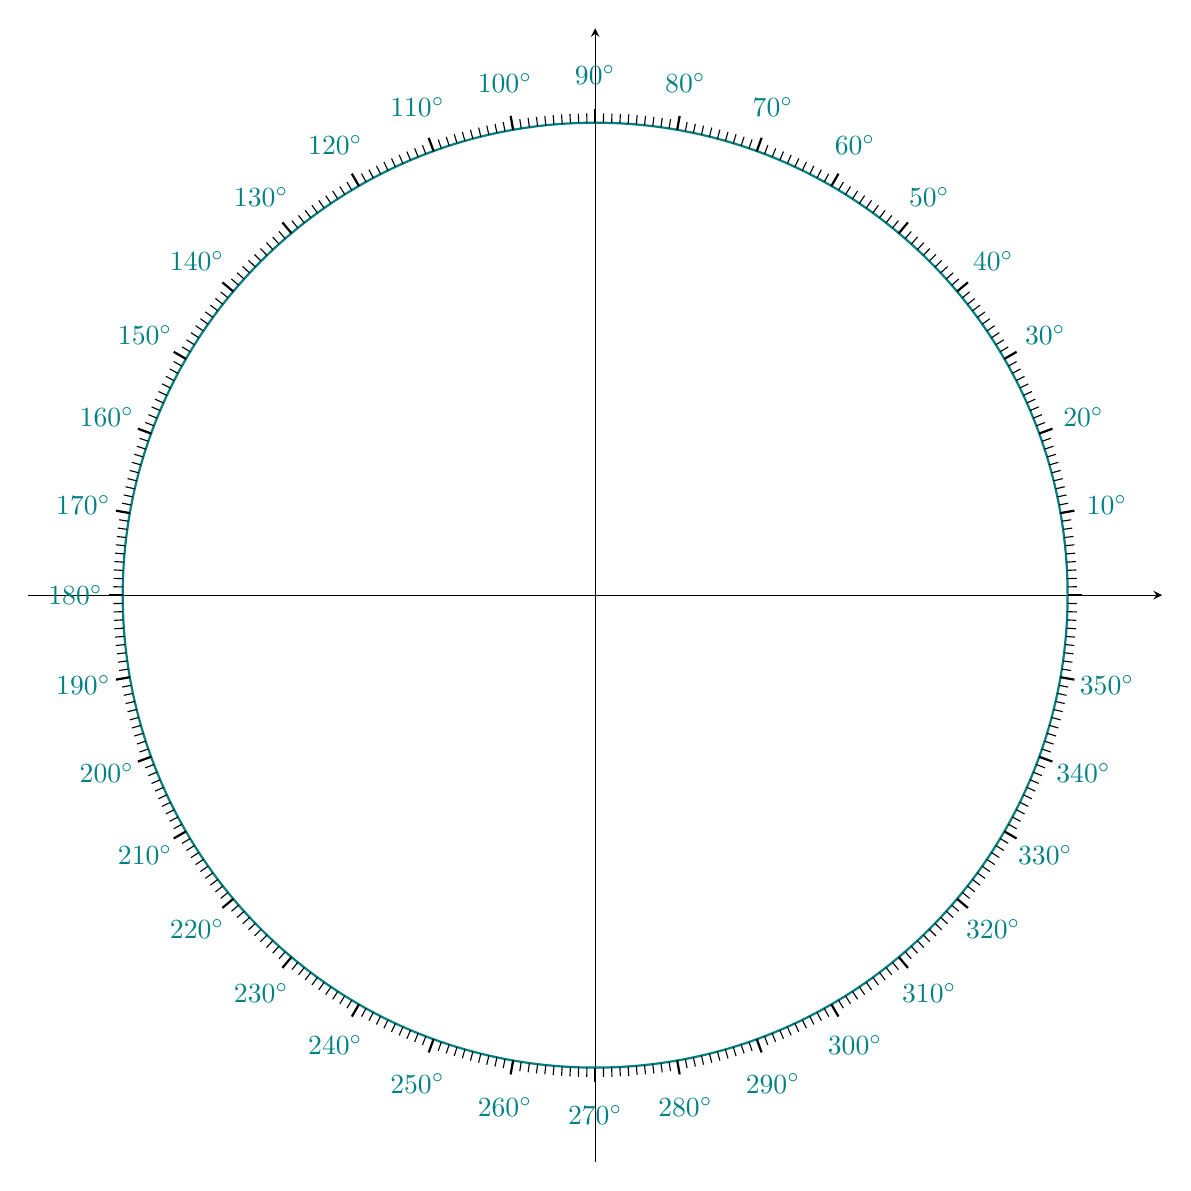
\begin{tikzpicture}
		\begin{axis}[
			axis lines = center, 
			xmin = -1.2, xmax = 1.2, 
			ymin = -1.2, ymax = 1.2, 
			x = 6cm, y = 6cm,
			ticks = none,
		]
			\draw[color = teal, thick] (axis cs:0,0) circle (6cm);
			%Ticks on circle 
			\pgfplotsinvokeforeach{0,1,...,35}
			{
				\draw[thick] (axis cs: {cos(#1*10)},{sin(#1*10)})-- (axis cs: {1.03*cos(#1*10)},{1.03*sin(#1*10)});
			}
			\pgfplotsinvokeforeach{10,20,...,350}
			{
				\node[color = teal] at (axis cs: {1.10*cos(#1)},{1.10*sin(#1)}) {$#1^\circ$};
			}
			\pgfplotsinvokeforeach{1,2,3,...,359}
			{
				\draw (axis cs: {cos(#1)},{sin(#1)})-- (axis cs: {1.02*cos(#1)},{1.02*sin(#1)});
			}
		\end{axis}
	\end{tikzpicture}
\end{center}
